\section{Le jeu de Lola (3 points bonus)}

Lola propose un jeu à ses deux amis, Juliette et Aurèle.

\begin{center}
	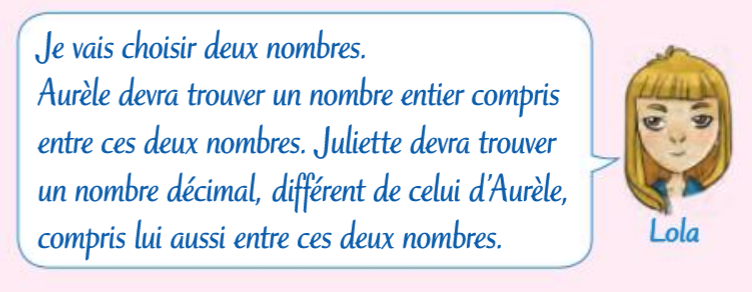
\includegraphics[scale=0.7]{img/lola}
\end{center}

\begin{questions}
	\question[1] Lola a choisi  \num{322.1} et \num{325.4}. Donner toutes les réponses possibles pour Aurèle et dix réponses possibles pour Juliette.
	
	\question[1] Lola choisi tà présent \num{12.3} et \num{12.4}. Donner toutes les réponses possibles pour Aurèle et dix réponses possibles pour Juliette.Peut-on donner toutes les réponses possibles ?
	
	
\question[1] Aurèle n'est pas content et dit à Lola que ses règles du jeu sont injustes. Expliquer pourquoi.
\end{questions}